\chapter{Second iteration}
\label{chap:second-iteration}
The second iteration was all about improving the issues outlined in the evaluation of the first iteration, this is also the final iteration in the project and leads to a complete product by the end. This chapter will include an analysis of the problems from the first iteration for the textual and visual elements, a description of how the design changed trying to solve these issues, how we implemented the changes and lastly an evaluation and what could be improved and what worked.
\section{Analysis and Design}
\label{chap:second-analysis}

\subsection{Textual analysis}
The biggest change in the second iteration is going from a hand-made/native solution to the use of external libraries. This change was done on the basis of some of the issues we ran into during the first iteration. For the textual element this includes the following table of issues:
% Please add the following required packages to your document preamble:
% \usepackage[table,xcdraw]{xcolor}
% If you use beamer only pass "xcolor=table" option, i.e. \documentclass[xcolor=table]{beamer}
\begin{table}[H]
\begin{tabularx}{\textwidth}{|l|l|X|}
\hline
\rowcolor[HTML]{9B9B9B} 
ID   & Name               & Description                                                                                                                                                                                                \\ \hline
\#01 & Extending the code & The issue with code extension was due to the fact that the entire code was written to handle one specific type of query and not a multitude of different queries (see more in first iteration chapter)     \\ \hline
\#02 & Error handling     & The error handling was not great as it was all custom written, meaning if there was an unforeseen error there would be no help for the user. This leads to frustration when you are a new user.            \\ \hline
\#03 & Code performance   & As mentioned in the evaluation of the first iteration there were issues with the performance of the code. The code was a collection of if-statements, which is quite inefficient for handling big queries. \\ \hline
\#04 & Maintainability    & Any bug in the code was close to impossible to identify as the code was written as long conditions for if-statements meaning that it could be hard to gage what is going on.                               \\ \hline
\#05 & Readability        & The readability was very poor. This meant it was difficult to for others to understand and potentially find bugs                                                                                           \\ \hline
\end{tabularx}
\label{tab:parser-issues}
\caption{The issues with the parser from the previous iteration}
\end{table}

To solve these issues, the group decided on the use of an external parser as it was an insurmountable task to solve all these issues with the current way of development. To help decide on a specific parser, the group made some evaluation criteria for how to rank the parsers from one another. This was helpful due to the lack of knowledge regarding the subject and no specific parser came to mind. The evaluation criteria are as follows:

% Please add the following required packages to your document preamble:
% \usepackage[table,xcdraw]{xcolor}
% If you use beamer only pass "xcolor=table" option, i.e. \documentclass[xcolor=table]{beamer}
\begin{table}[H]
\begin{tabularx}{\textwidth}{|l|l|X|}
\hline
\rowcolor[HTML]{9B9B9B} 
ID   & Name           & Description                                                                                                                                                                                                                                                                                                                                                                                                                                                                                                                                                                         \\ \hline
\#01 & Error handling & \begin{tabular}[c]{@{}X@{}}The number one priority for the parser was to have great error handling as our software is targeted towards new users. To be able to see where they are going wrong is the single most important thing.\\ To give a metric on how to evaluate error handling we made a list of error handling features it should include:\\ 
\begin{minipage}[t]{0.65\textwidth}
    \begin{itemize}
    \item Knowing what the errors, including the expected result ie. Found “x” expected “y”
    \item   Knowing where the error is, to allow for line number and highlighting ie. Error on line 32, character 5\\
    \end{itemize}
  \end{minipage}    
    \end{tabular} \\ 
    \hline
\#02 & Ease of use    & \begin{tabular}[c]{@{}X@{}}As said the group has little to no experience working with a parser or similar technology so ease of use would rank highly as we have limited time to learn an entire new technology and did not think it was a valuable use of our time.\\ The metrics for the ease of use are as follows:      
\begin{minipage}[t]{0.65\textwidth}
    \begin{itemize}
    \item Parse generation means that we do not have to write code but can just write rules.
    \item   An online editor or examples to play around with when learning the parser\\
    \end{itemize}
  \end{minipage}    
    \end{tabular} \\ 
    \hline
\#03 & Performance    & The last evaluation criteria is the performance of the parser. The reason for this being the least important is due to the target demographic mainly using our software as a stepping stone. This means they will most likely not use it for bigger projects as that is not the intended use and there are better solutions for that. Performance can be a more specific metric than the other criterias, as you can put a number deciding fast it should be able to process a worst-case scenario.                                                                                 \\ \hline
\end{tabularx}
\label{tab:parser-issues}
\caption{Evaluation criteria for the textual parser}
\end{table}

To gather a list of potential parsers to use, the group found the following website: https://chevrotain.io/performance/.This website contains benchmarks and comparisons for 11 different parsers. These comparisons are done on “an input sample of an around 1000 lines JSON file”\cite{parsePerformance}. As this is a benchmark test it is only ranked in terms of performance, see below for full rankings. The group is aware of the potential bias in these rankings as the site ranks the parser the site is built around.  This does not play a big role as it was mostly used to gather a list of parsers and not as much the performance aspect of each parser.
To rank the other two categories, an analysis was made as seen in the table below:

% Please add the following required packages to your document preamble:
% \usepackage[table,xcdraw]{xcolor}
% If you use beamer only pass "xcolor=table" option, i.e. \documentclass[xcolor=table]{beamer}

\begin{table}[H]
\begin{tabularx}{\textwidth}{|l|l|X|X|}
\hline
\rowcolor[HTML]{9B9B9B} 
ID & Name       & Error handling                                                                                                                                  & Ease of use                                                                                                                                  \\ \hline
01 & Chevrotain\cite{ChevrotainGithub} & Good error handling with some decent highlighting of where things go wrong. Has all the features we are looking for in terms of error handling. & No parse generation, meaning we have to write the code for the parser itself which is a big hassle. A good online editor nothing too special \\ \hline
02 & ANTLR4\cite{ANTLRGithub}     & Requires some work to get the error handling we want                                                                                            & No online editor and quite challenging grammar structure                                                                                     \\ \hline
03 & Parsimmon\cite{ParsimmonGithub}  & Requires a bit of work to get a readable error text, but includes both features                                                                 & No online editor, and no parse generation                                                                                                    \\ \hline
04 & PEG.js\cite{PEGJSGithub}     & Really good error handling provides everything we want                                                                                          & A great online editor and easy to understand and play with grammar                                                                           \\ \hline
\end{tabularx}
\caption{}
\label{}
\end{table}

The rest of the entries were lacking behind PEG.js in all three categories and we therefore did not find it necessary to include them in this table. In the end the decision to go with PEG.js was made as the parser of choice due to it having the best combination of error handling and ease of use, and even with the quite low ranking in performance it is still more than fast enough to process the data we need for this solution. 



\subsection{Visual analysis}
To fix the issues regarding the visualization, which was outlined in the evaluation of the 1st iteration, the decision landed on using an external library for the visualisation. The chosen library was D3.js. D3.js is a visualisation library that helps creating visualisations in fewer and, and probably more efficient, lines of code\cite{useD3}.  D3.js is also a library that the group has come across several times in resolving SVG related issues. D3.js is one of the most popular visualisation tools for JavaScript, and this leads to a great amount of documentation in the form of tutorials, video guides, premade examples, and Q\&As. The huge amount of documentation did however turn out to cause some confusion at times as D3.js comes in different versions with previous version methods becoming obsolete and faced out. It was therefore of huge importance to ensure the right documentation version was found when working with D3. D3 is also very modular, and the necessary modules can be imported, setting up for shorter load times.
A big factor in switching to a library such as d3.js, was the implemented force layout in iteration one. As mentioned in the evaluation, the force implementation was rough looking and took time to settle. In d3.js, force is a module which can be imported, and a force directed graph is quite common to find in d3 documentation\cite{forcedirectedD3}.

\subsection{Design}
The use of external libraries allowed us to simplify the design greatly, as we could remove some of the external classes and simplify the methods in the kept classes.

\begin{figure}[H]
    \centering
    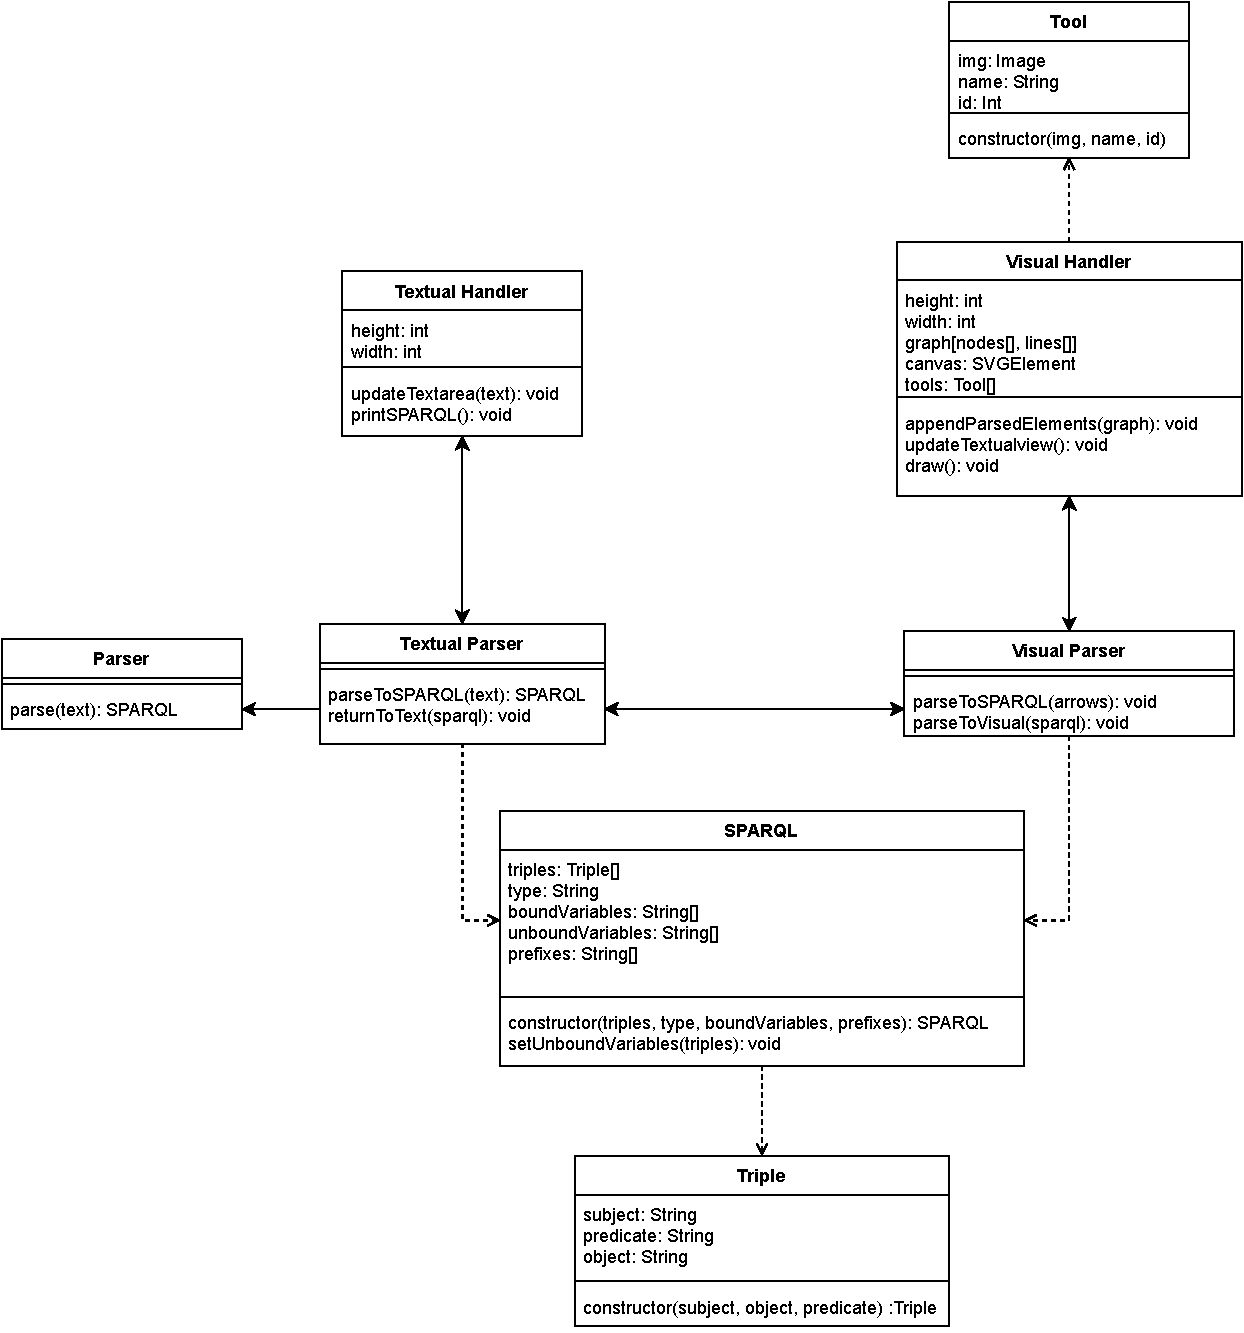
\includegraphics[angle=90,origin=c,width=1.3\textwidth]{figures/2nd_iteration_design.pdf}
    \caption{Caption}
    \label{fig:my_label}
\end{figure}

The way the design changed from the first to the second iteration is the removal of the nodes and arrows objects, as they are no longer needed since they are already being featured in D3.js. This also meant changing from an array of nodes and an array of arrows to a single multi dimensional array. The only thing added during this process has been the parser class
\section{Implementation}
\subsection{Textual Implementation}
The implementation of the textual parser was quite different from the previous work as it now relied on grammar instead of actual JS code. An example of the difference can be seen in figure \ref{fig:pegjs} below:
\begin{figure}[H]
    \centering
    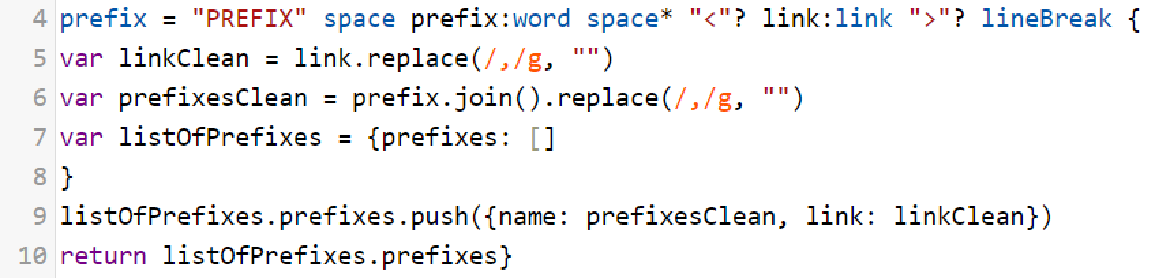
\includegraphics[width=1\textwidth]{figures/pegjs.pdf}
    \caption{Picture of prefix code for parser}
    \label{fig:pegjs}
\end{figure}
Figure \ref{fig:pegjs} also highlights the unforeseen issue we had with the PEG.js parser. The parser returns char arrays instead of strings leading to the strange join and replace functions seen.

\bigskip
The way a parser like this works is by giving it some kind of grammar it can read through and some text. It will then return different objects from the text depending on the grammar. The way this particular parser works is by defining a set of rules. Looking at the example in figure x.x, a prefix is defined as the word PREFIX in all caps followed by a space, then a word which we give the name prefix, so we can refer back to value later, yet another space with an asterix indicating that there can be between 0 and many spaces, then followed by a “<” with the question mark meaning that it does not have to be there but could be, then a link with the name link, another > with a question mark and lastly a line break. This all leads to us being able to grab the two things we gave names to and return as a prefix object when the parser is called. The parser then uses this grammar to create a massively complicated JavaScript file that is the parser itself and the one that runs in our code but we do not have to ever touch this file as its all auto generated so we can just call the parse function and it runs according to the grammar it was created with.

\bigskip
The error handling also changed a lot during the second iteration as the parser used had inbuilt error handling, so we just had to get the message and location to display it in the error handling box. We wanted to implement some highlight of where the error was to make it easier to pinpoint but since HTML does not natively support highlighting in textareas we had to implement the jQuery library called “highlight textarea” this is a quite simple library that allows you to highlight the text of a textarea by giving it either words to highlight or a range to highlight, since the error handling from the parser already include a range of the error this was the obvious choice see figure \ref{fig:errorhandling}:
\begin{figure}[H]
    \centering
    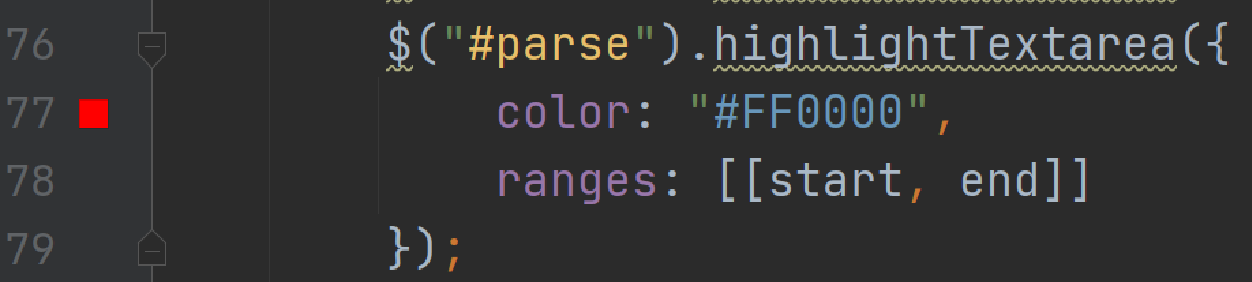
\includegraphics[width=1\textwidth]{figures/errorhandling.pdf}
    \caption{Error handling highlighting}
    \label{fig:errorhandling}
\end{figure}
As can be seen on figure \ref{fig:errorhandling} this is a simple process you just have to give the ID of the textarea and call the highlightTextarea function that takes a colour in this case red to indicate that is an error and the range in this case the start and end of our error.

\subsection{Visual Implementation}
The second iteration led to the implementation of the library D3.js and a couple of new functionalities for the visualisation, see figure \ref{second-iteration-ui}. When implementing d3, the two classes, Node and Arrow, could be removed from the application. The visualisation is now stored in a graph variable containing both nodes and lines, figure \ref{graph}.

\begin{figure}[H]
    \centering
    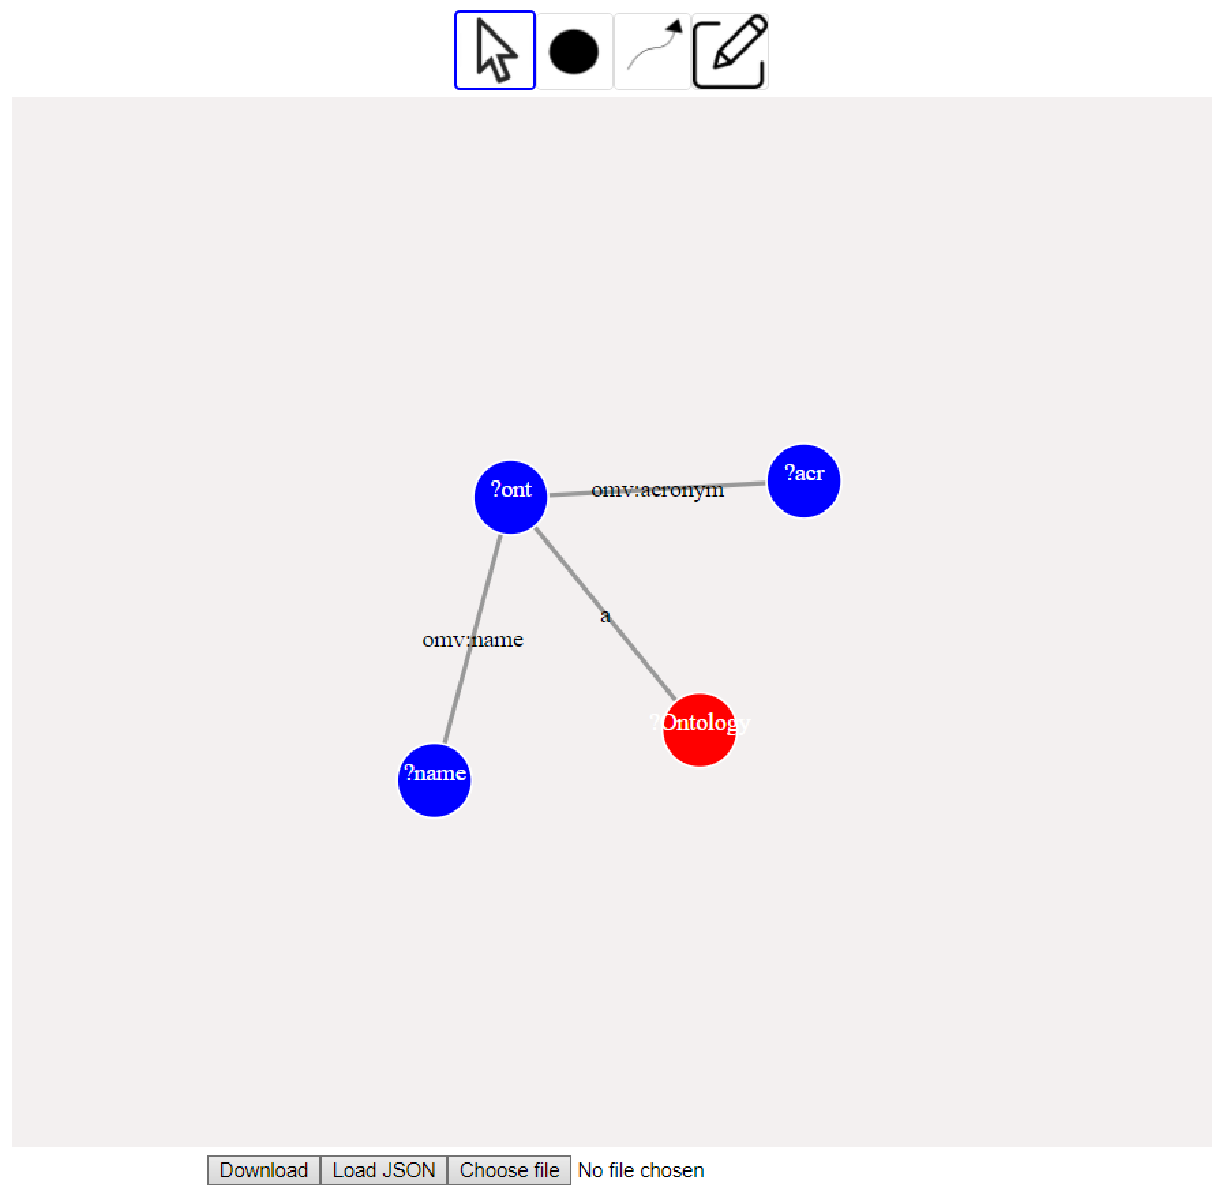
\includegraphics[width=1\textwidth]{figures/second-iteration-ui.pdf}
    \caption{Visual part in the second iteration}
    \label{fig:second-iteration-ui}
\end{figure}

\begin{figure}[H]
    \centering
    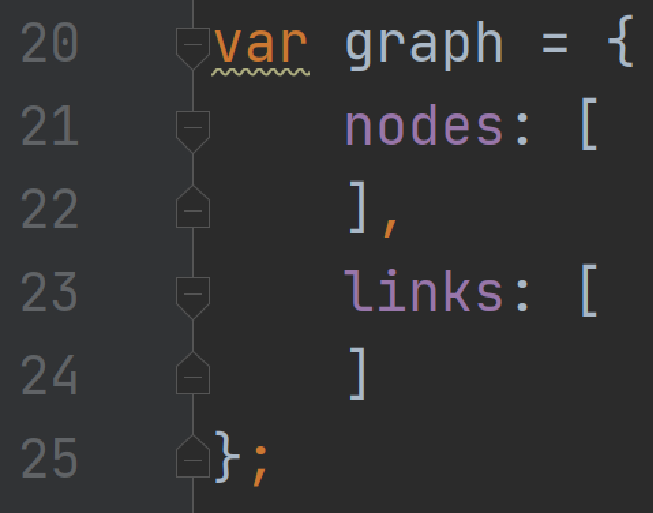
\includegraphics[width=0.5\textwidth]{figures/picture-graph.pdf}
    \caption{The graph variable storing the visualisation}
    \label{fig:graph}
\end{figure}

With the implementation of d3.js, a new version of the force directed graph has been implemented, see figure \ref{fig:forceimplementation}. The written code for the force simulation is significantly shorter than the one implemented in the first iteration, and the second implementation has noticeably more options. As seen on lines 271-274, different attributes of the simulation have been set. These attributes can help push the visualisation toward the centre of the canvas, add collision between the nodes so that they do not overlap, and add a charge to all nodes to push them away from each other. This force simulation is also a part of a bigger draw method, which can easily be called when wanting to update the visualisation. This makes for significantly easier implementation when wanting to add new SVG elements to visualisation. All required of the developer is to add a new group to the draw method, see figure \ref{fig:addednode}. Here the code resembles normal SVG implementation, with the addition of the d3 drag module, line 310-311. This module gives the visualisation the required methods to become more dynamic and draggable by the user.

\begin{figure}[H]
    \centering
    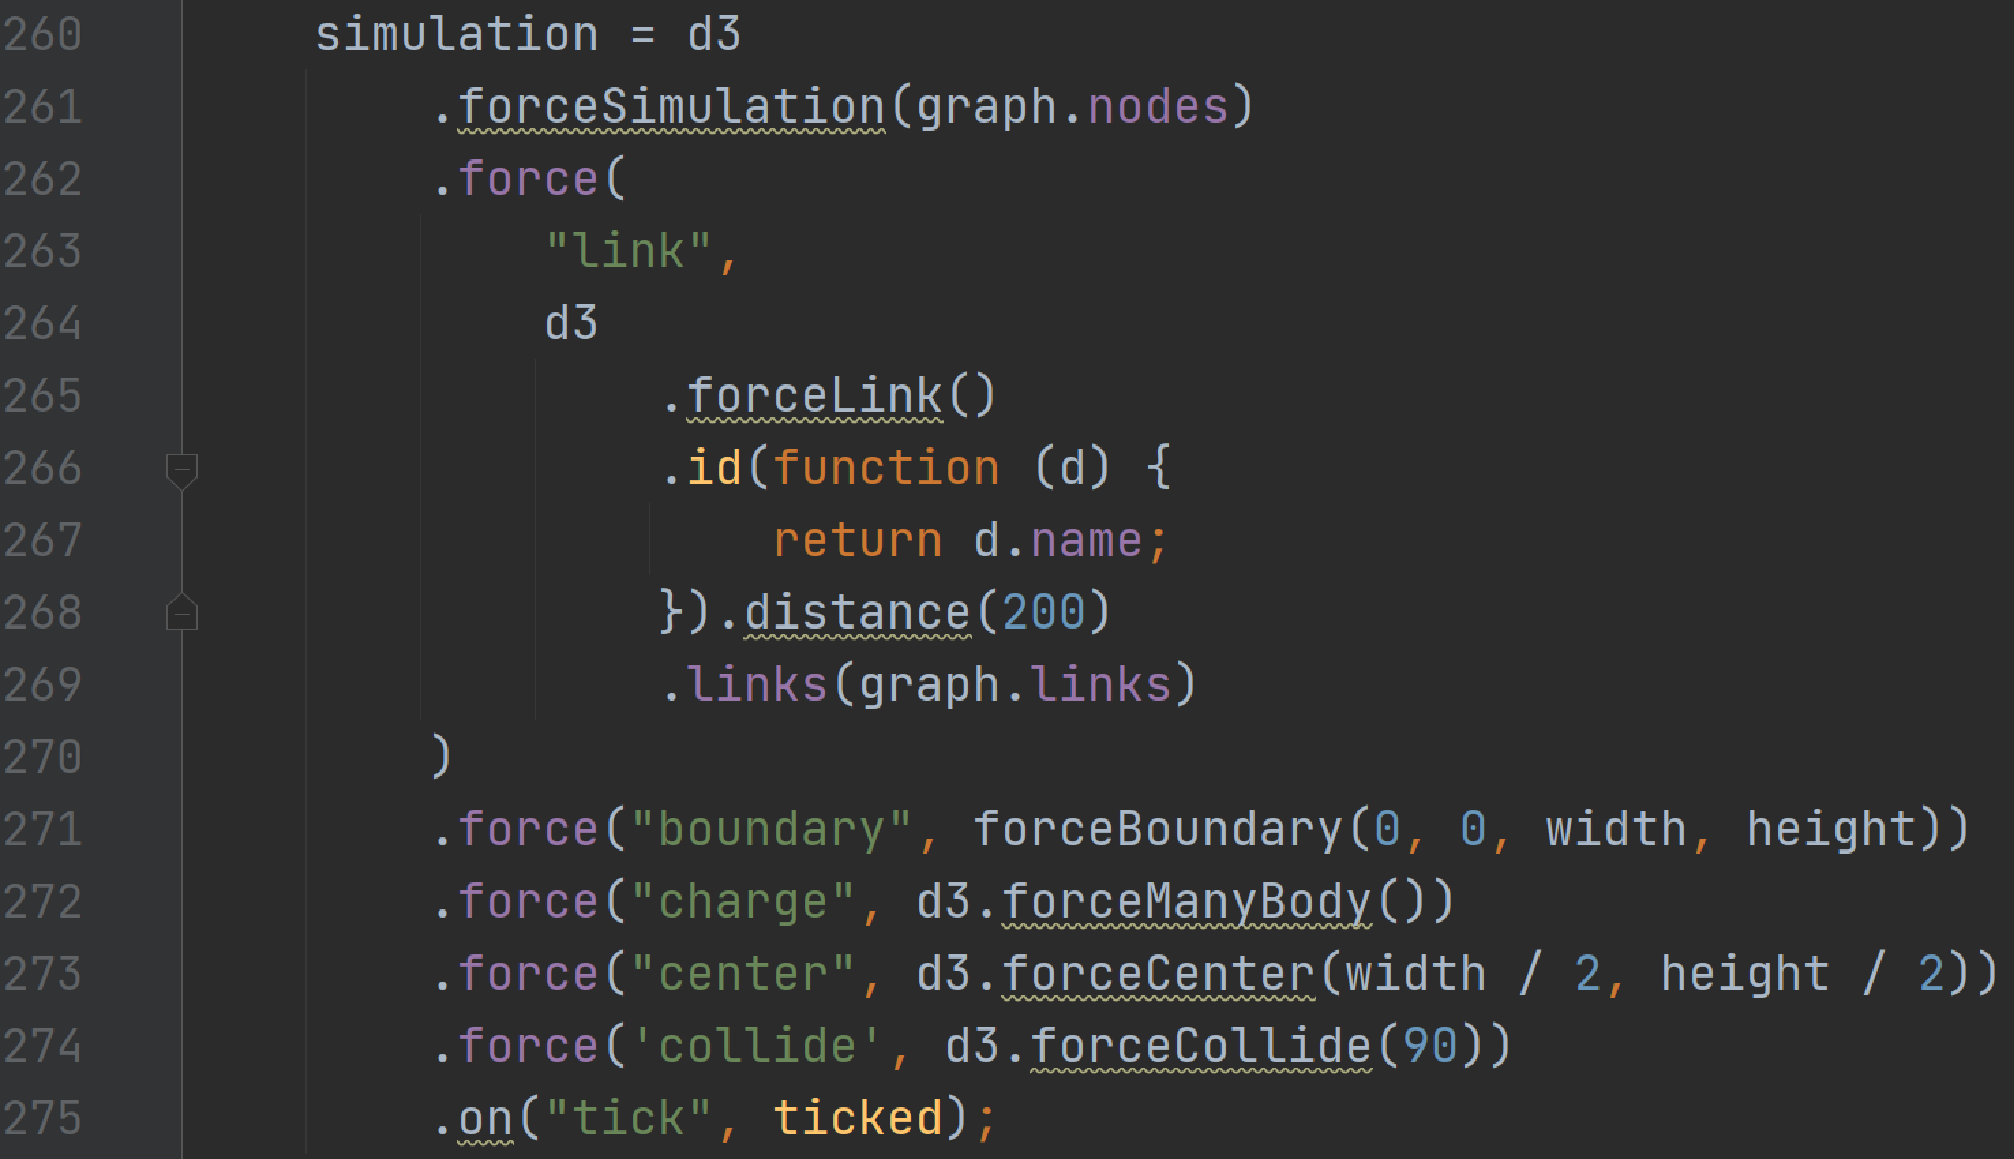
\includegraphics[width=1\textwidth]{figures/force-implementation.pdf}
    \caption{Force implementation with D3.js}
    \label{fig:forceimplementation}
\end{figure}

\begin{figure}[H]
    \centering
    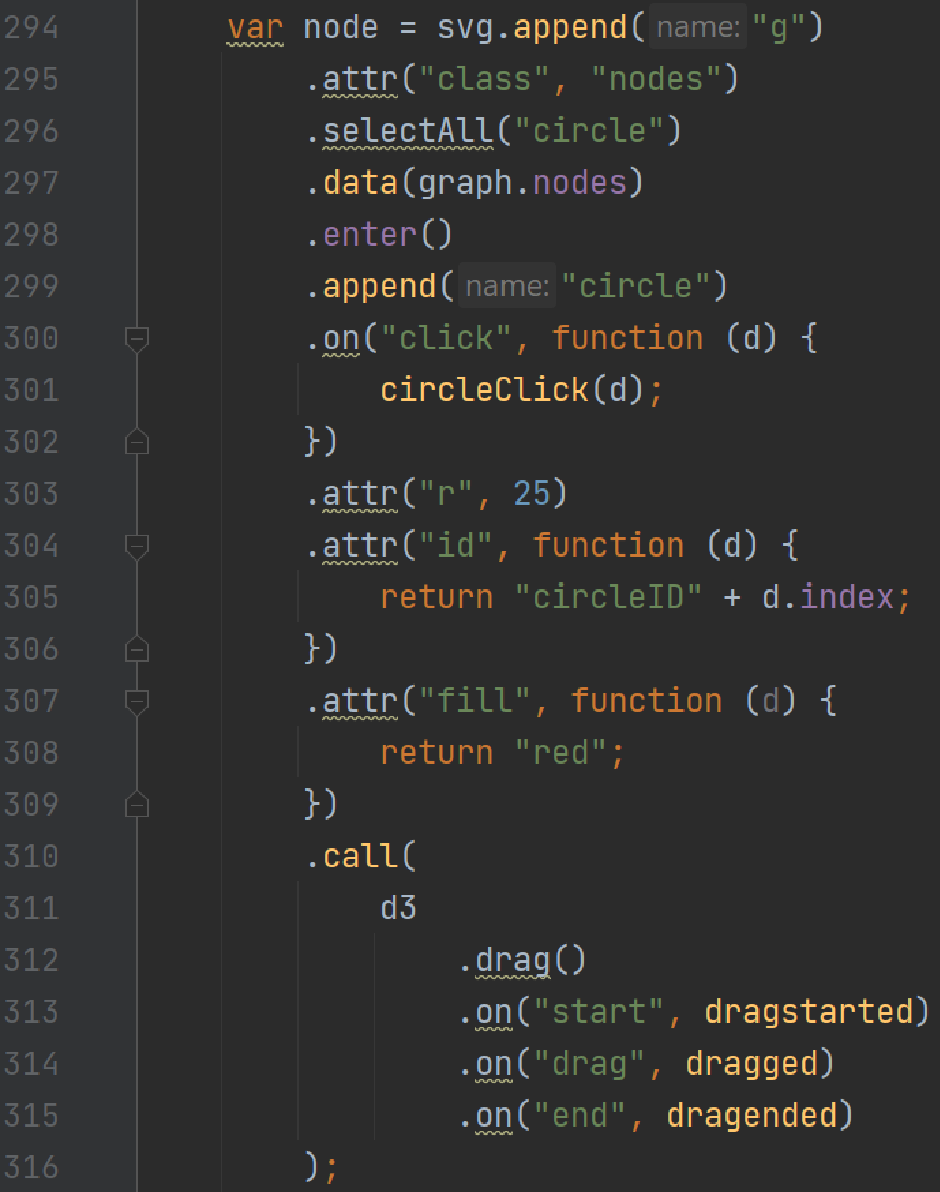
\includegraphics[width=0.8\textwidth]{figures/added-node.pdf}
    \caption{Added node}
    \label{fig:addednode}
\end{figure}

Some of the requirements implemented into this iteration was the ability to download and load the visualisation, see figure \ref{fig:second-iteration-ui}. The group discussed which file format the downloaded file should be, and it ended with a choice of JSON. While JSON does not offer the possibility to view the visualisation as an image, it has easy implementation when converting from the graph variable seen in figure \ref{fig:graph}. JSON also allowed for a simple implementation when uploading which perhaps would have been much more difficult with a file type like JPEG or PNG.
\\
Lastly, a new tool has been added, figure \ref{fig:second-iteration-ui}. The added tool fills the requirements of editing the nodes and arrows. The tool opens the same popup as the creation tools but this time it inputs the selected elements information. In figure \ref{fig:edittool} the edit tool can be seen used on a bounded node called “?name”.

\begin{figure}[H]
    \centering
    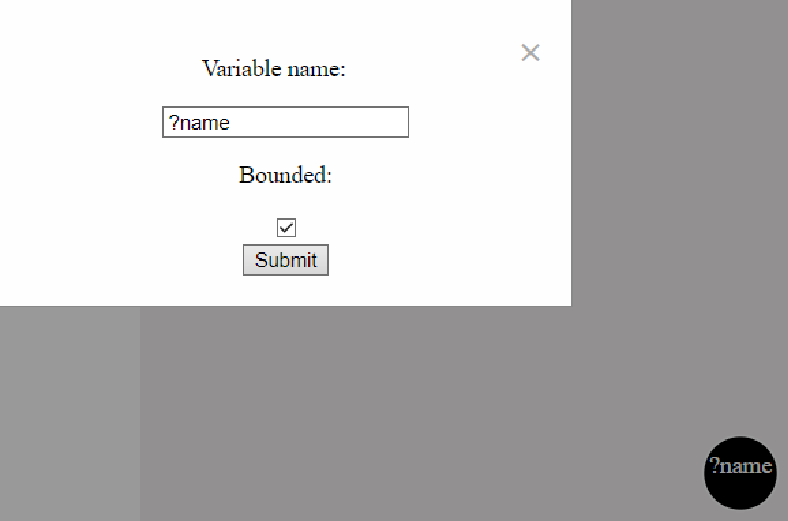
\includegraphics[width=1\textwidth]{figures/edit-tool.pdf}
    \caption{The edit tool in action}
    \label{fig:edittool}
\end{figure}

\section{Testing}
\begin{figure}[H]
    \centering
    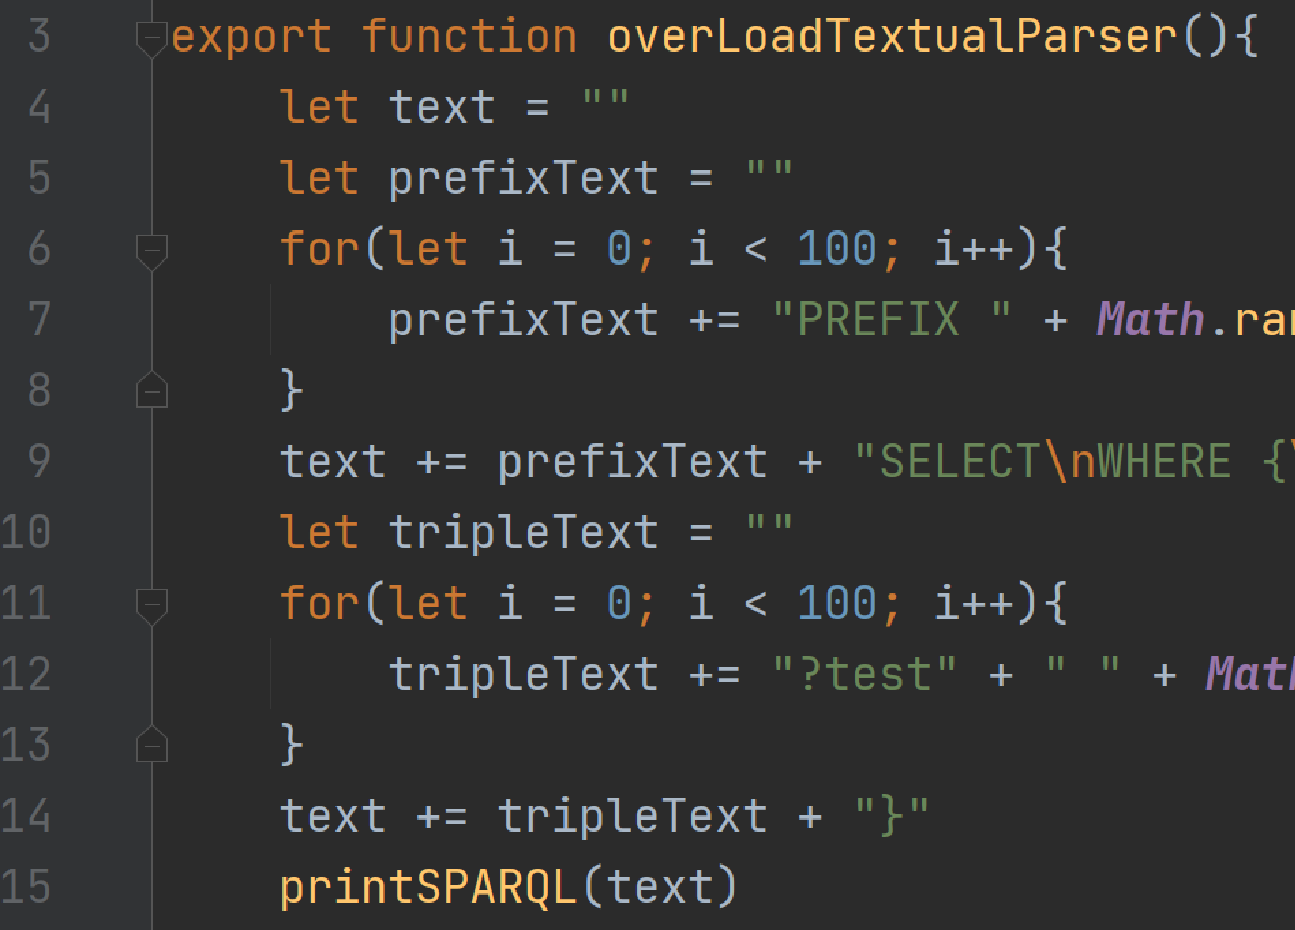
\includegraphics[width=1\textwidth]{figures/overloadgeneration.pdf}
    \caption{Function for overloading both the visual and textual element}
    \label{fig:overload}
\end{figure}
Figure \ref{fig:overload} is a showcase of a function that creates 100 prefixes and 100 triples. This is done to create such a big query that we will never expect a user to input this much data, and can be used as an absolute worst case scenario. The figure \ref{fig:time-forloop} shows the way we went about getting time data and how we ran the test. It's as simple as running the test 100 times and logging when the function started and when the function ended.
\begin{figure}[H]
    \centering
    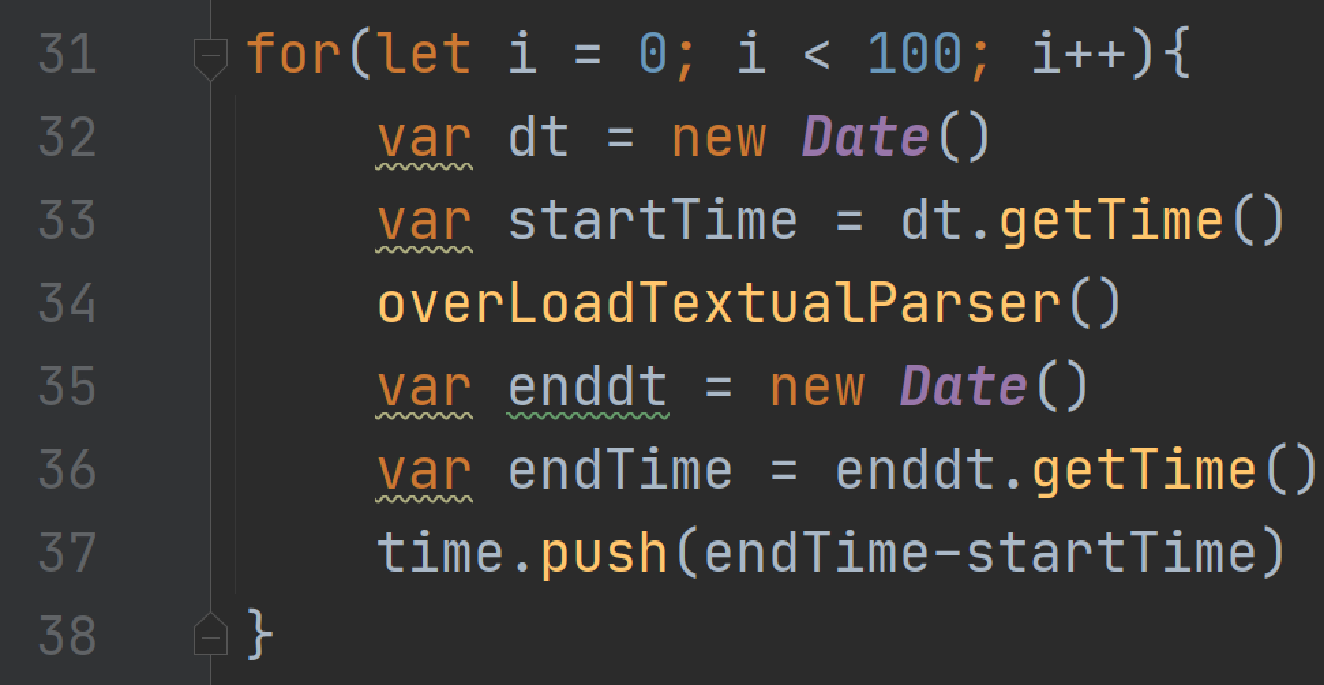
\includegraphics[width=1\textwidth]{figures/time-forloop.pdf}
    \caption{For loop to get the time from start to finish of the overload function}
    \label{fig:time-forloop}
\end{figure}
Figure \ref{fig:array-15} shows the time in milliseconds for the first 15 runs and as can be it is all done within 100ms which was the goal for our performance. 
\begin{figure}[H]
    \centering
    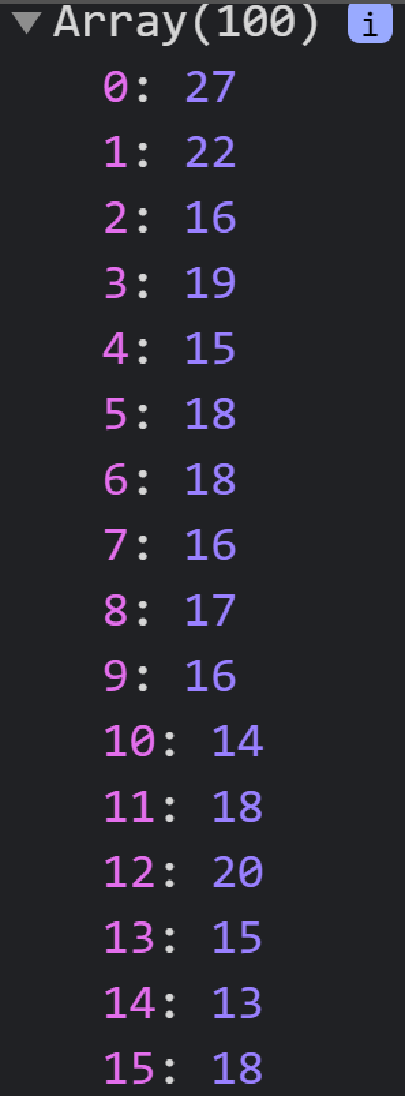
\includegraphics[width=0.2\textwidth]{figures/array-15.pdf}
    \caption{Array showcasing the first 15 times}
    \label{fig:array-15}
\end{figure}
Figure \ref{fig:bad-visual} shows how the visual element handles it and as can be seen it gets quite overloaded and can’t figure where to place things this is in part due to the query being 100 different pairs of nodes being showcased meaning there is simply not enough space on the canvas size chosen, however this is not a big issue as this is way more than a realistic query would like.
\begin{figure}[H]
    \centering
    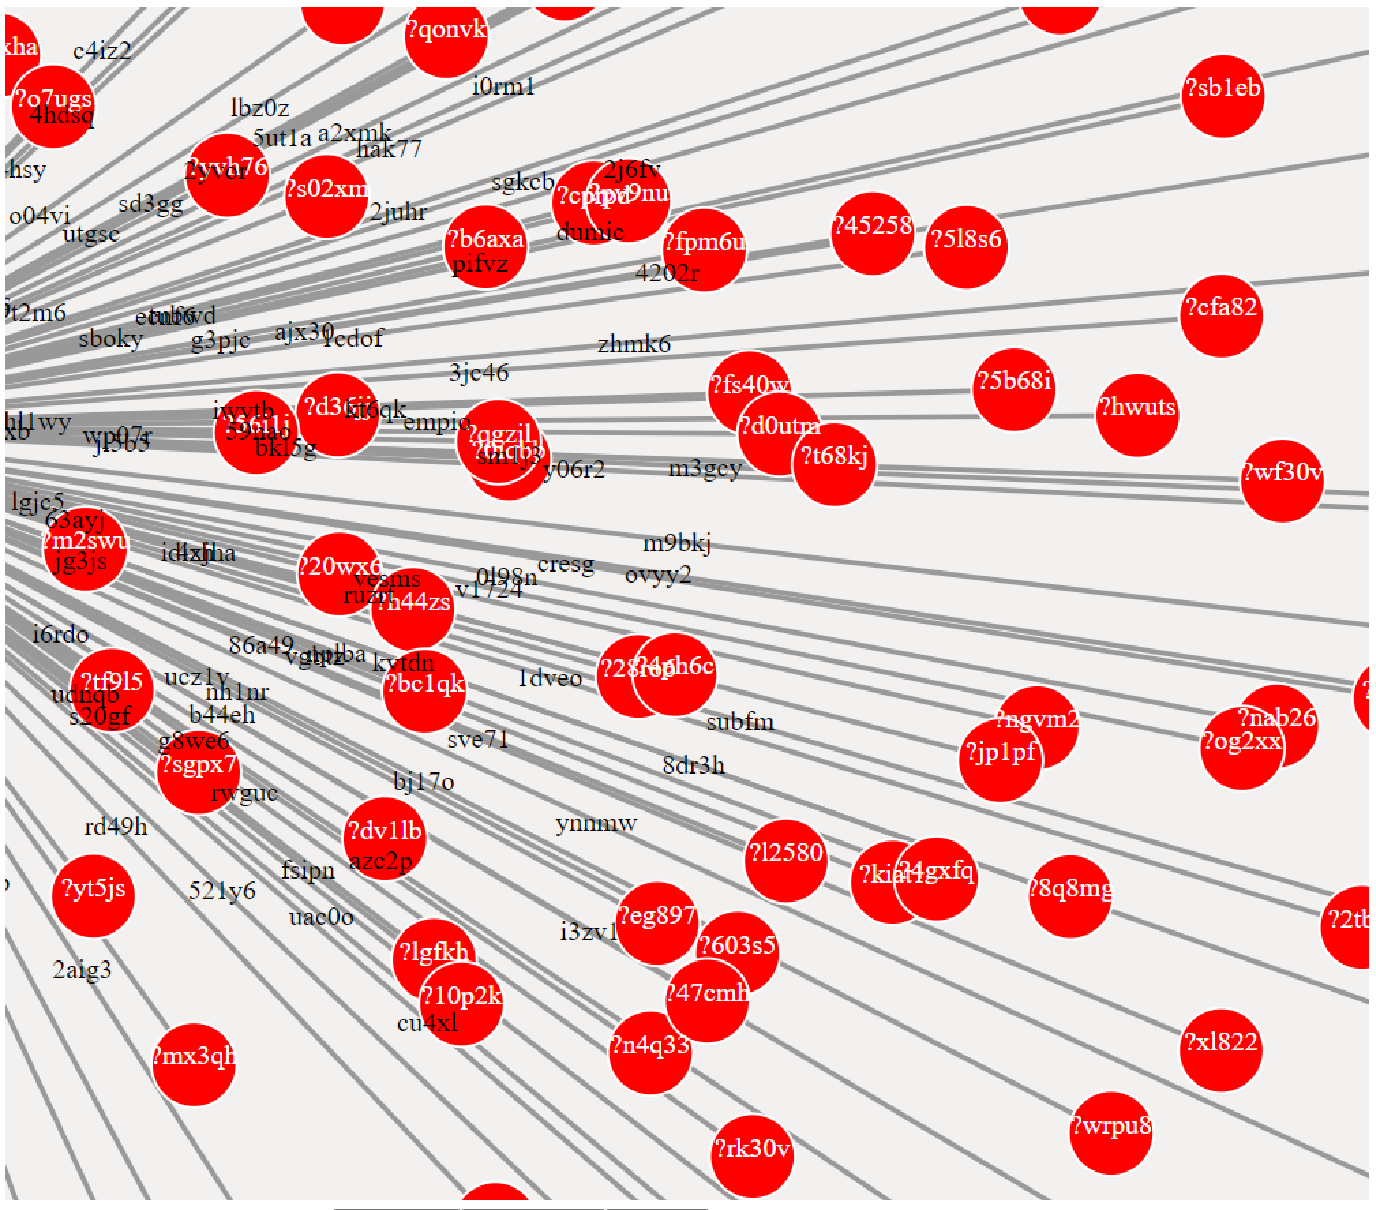
\includegraphics[width=1\textwidth]{figures/bad-visual.pdf}
    \caption{The visual element being under stress}
    \label{fig:bad-visual}
\end{figure}



\section{Evaluation}
\label{chap:second-eval}
When it comes to the textual part of the second iteration, it was a difficult task at hand since we had no experience working with any kind of parser technology. This led to a lot of time spend in the online editor of the parser trying to figure out how does it work and how do we make sure it can handle everything we want, this meant a lot of changes in the grammar along the way and many small bug fixes each taking up anywhere from 1min to multiple hours trying to solve. We also tried to implement some continuous updating, but sadly we could not figure out how to make any of it not annoying when writing the query, as there were some issues with HTML textareas that when you update it unfocuses the textarea meaning the cursor gets put back at the start. Luckily, we managed to fix this issue by a workaround, this just led to the issue of highlighting or error messages getting in the way when trying to type as we figured obviously while typing you do not expect the half-finished work to be error free and therefore, we landed on the click of a button or manually unfocusing the textarea was the best solution. We wanted to implement a way to highlight variables in the query like seen in the “NITELIGHT EXAMPLE'' and figured we would use the same highlight library as before, unfortunately this is library does not support dynamic updates of the code meaning we would write a function for each number of potential variables, we figured this was a solution that scaled so badly that we scrapped the idea.

\bigskip
The visual implementation for the second iteration handled a few requirements not completed in the 1st iteration. While some of those requirements were functional, the focus of this iteration has been with the non-functional requirements. This meant that with the implementation of the library d3.js, there has been significant improvements to the visualisation part. With d3s already implemented force simulation, the force directed graph from the 1st generation has become noticeably smoother and more appealing to look at. D3.js also helped give new functionality by making the nodes draggable. Lastly, d3 has been the codebase more friendly towards further development.
\bigskip
There was not a lot of new functionality for the user in the second iteration, and while this may seem regrettable, there are still significant improvements to the application. The codebase has been significantly improved, making it easier to continue development in later stages, and the already existing functionality has also improved notably, making it a more appealing program. The application is now completely ready for a potential 3rd iteration, which would be an appreciably easier iteration. A potential 3rd iteration would come with a huge functionality boost by simply adding to the already existing library implementations. Especially the parser would see easy implementation as new rules can be added to the grammar file to implement new functionality.